\section{段階的な自己開示による受容性の向上可能性}

\ref{研究課題と仮説}節では「カラオケ空間における音楽嗜好の段階的な自己開示が的受容性に及ぼす影響」を研究課題として設定した．本節ではその研究課題に伴う3つの仮説について，結果を述べる．


\subsection{仮説1の結果}\label{仮説1の結果}

\ref{研究課題と仮説}節で述べた仮説1「低いレベルから高いレベルへと段階的に自己開示を行うことで，深いレベルの自己開示に対する受容度が高くなる」について検証を行うため，システムによる選曲履歴データと実験中のアンケート結果を分析した．選曲履歴からの自己開示レベルの推移を図\ref{fig:自己開示レベルの推移}に示す．段階的な自己開示を促進した推薦あり群は設計通りの段階的な上昇（フェーズ1の約1.0から最終フェーズの約3.5まで）を示した．一方，推薦なし群は比較的一定のレベル（約2.5）を維持していた．この結果は，システムの介入が意図した通りに機能したことを示している．

\begin{figure}[H]
    \centering
    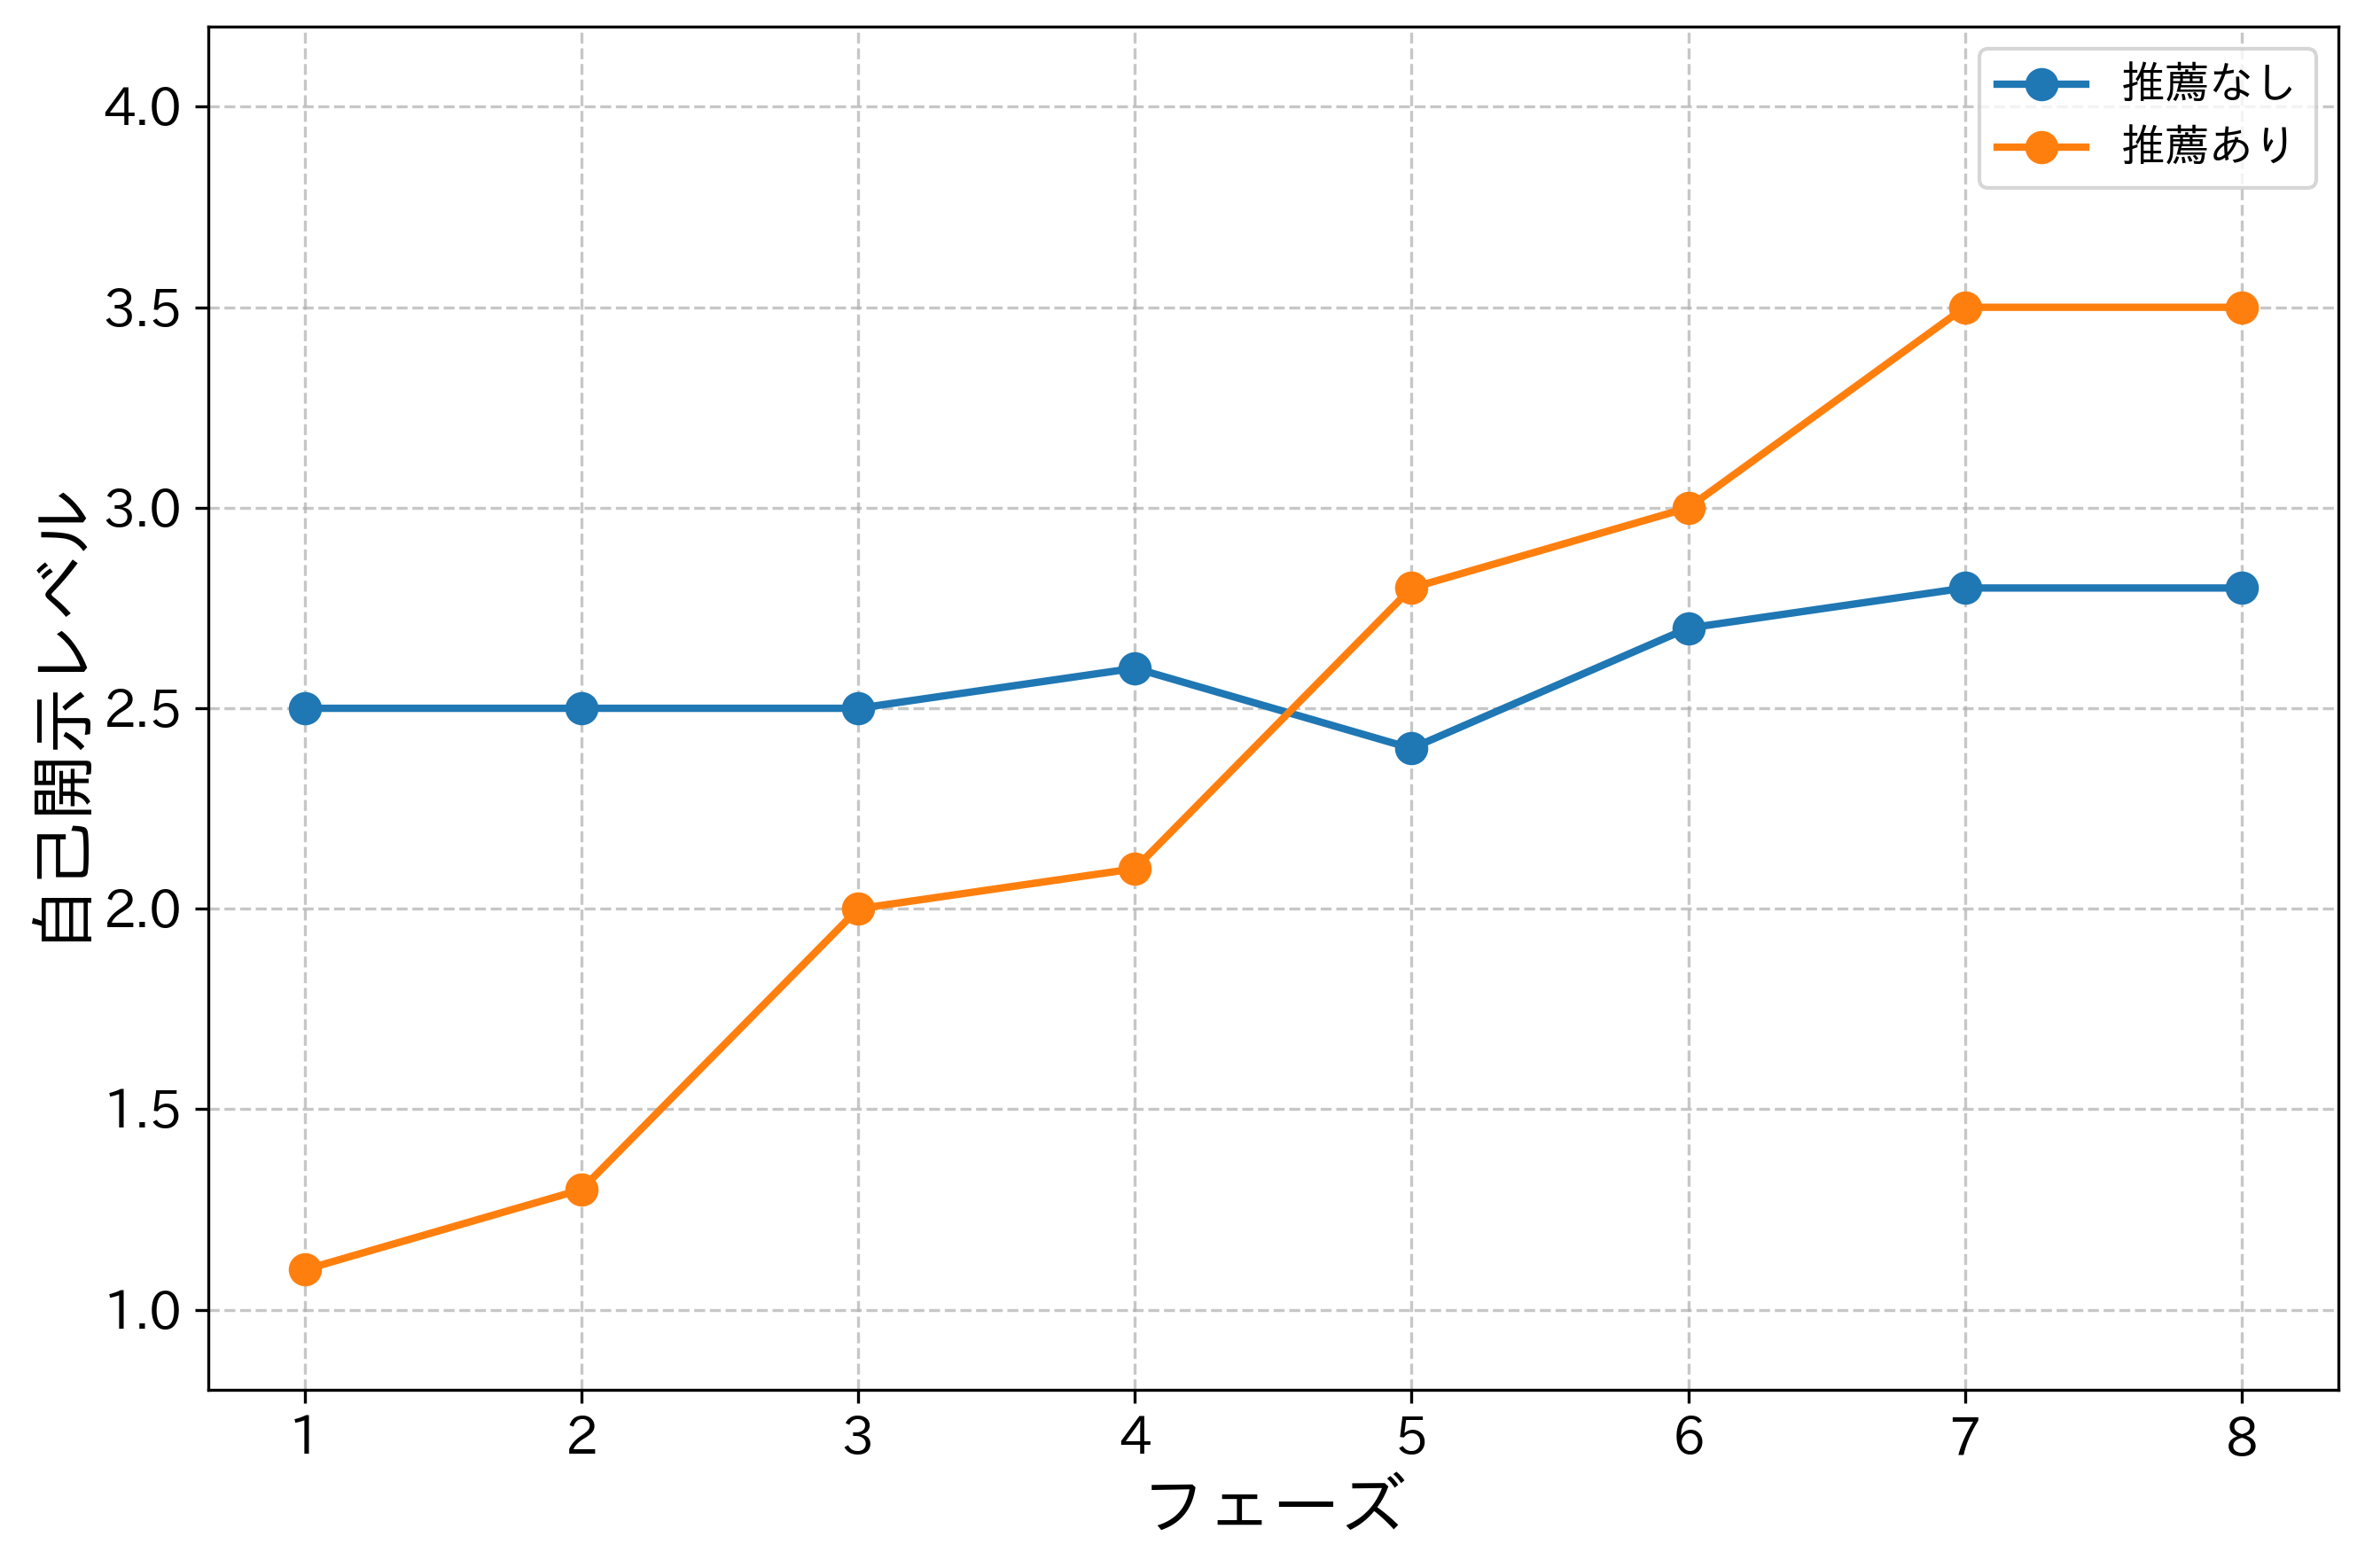
\includegraphics[width=0.9\linewidth]{image/自己開示レベル推移.png}
    \caption{自己開示レベルの推移}
    \label{fig:自己開示レベルの推移}
\end{figure}

実験中のアンケート結果の時系列変化を図\ref{fig:Q5}, 図\ref{fig:Q6}に示す．EQ5（聴いた曲について楽しく話ができた）に関しては，フェーズ5, 6で一時的にスコア4を下回る傾向が見られたものの，最終フェーズ（7, 8）ではレベル3, 4の深い自己開示が行われた状況下でも高い受容度を示した．EQ6（思いや経験が理解できた）の結果からも，推薦あり群は推薦なし群と顕著な差異を示すことなく，特にフェーズ1〜4と7〜8において近似した値を示した．これは，段階的に自己開示を促し深いレベルに到達した場合でも，推薦をしていない群の自己開示と同等の受容度を維持できることを示唆している．具体例として，ユーザーJやKは自己開示レベル4まで到達しながらも，実験開始時からの高い受容度を維持し続けた．

推薦あり群が後半フェーズ（5〜8）で深い自己開示を促されているにも関わらず，推薦なし群と同等の高い受容度を維持していることが確認された．

\begin{figure}[H]
    \centering
    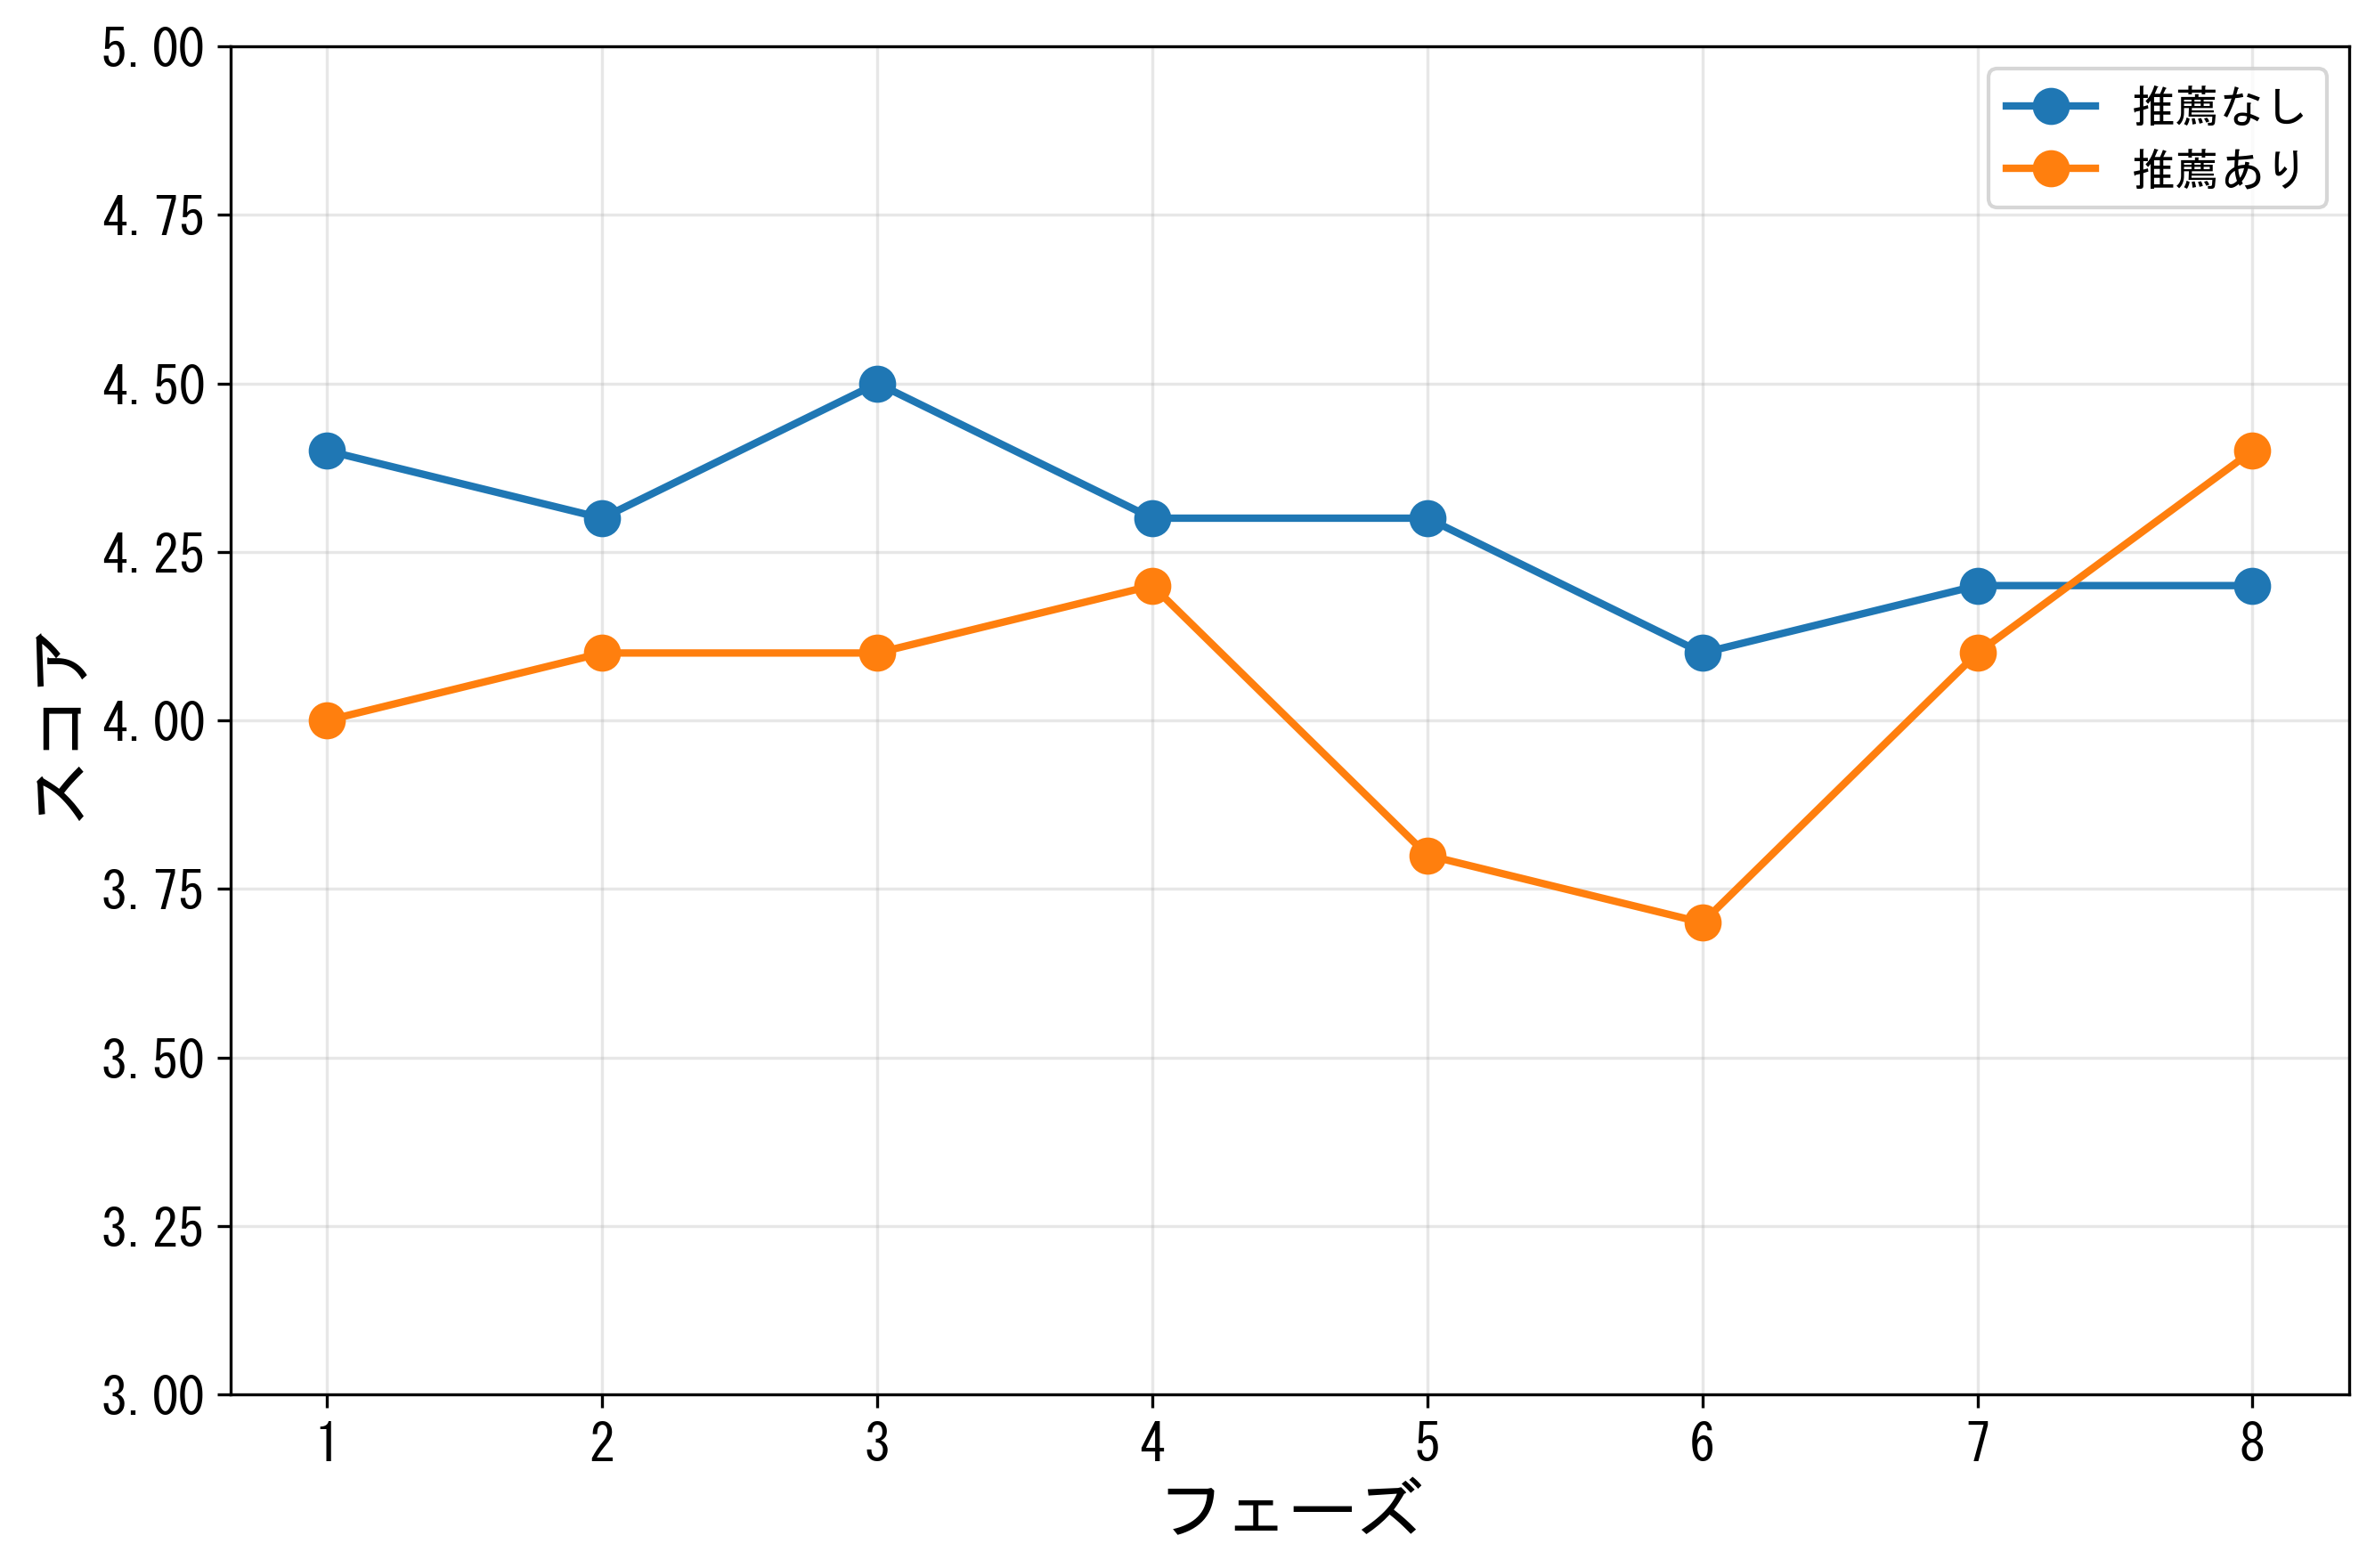
\includegraphics[width=0.9\linewidth]{image/Q5の平均推移.png}
    \caption{EQ5: 聴いた曲について楽しく話ができた}
    \label{fig:Q5}
\end{figure}

\begin{figure}[H]
    \centering
    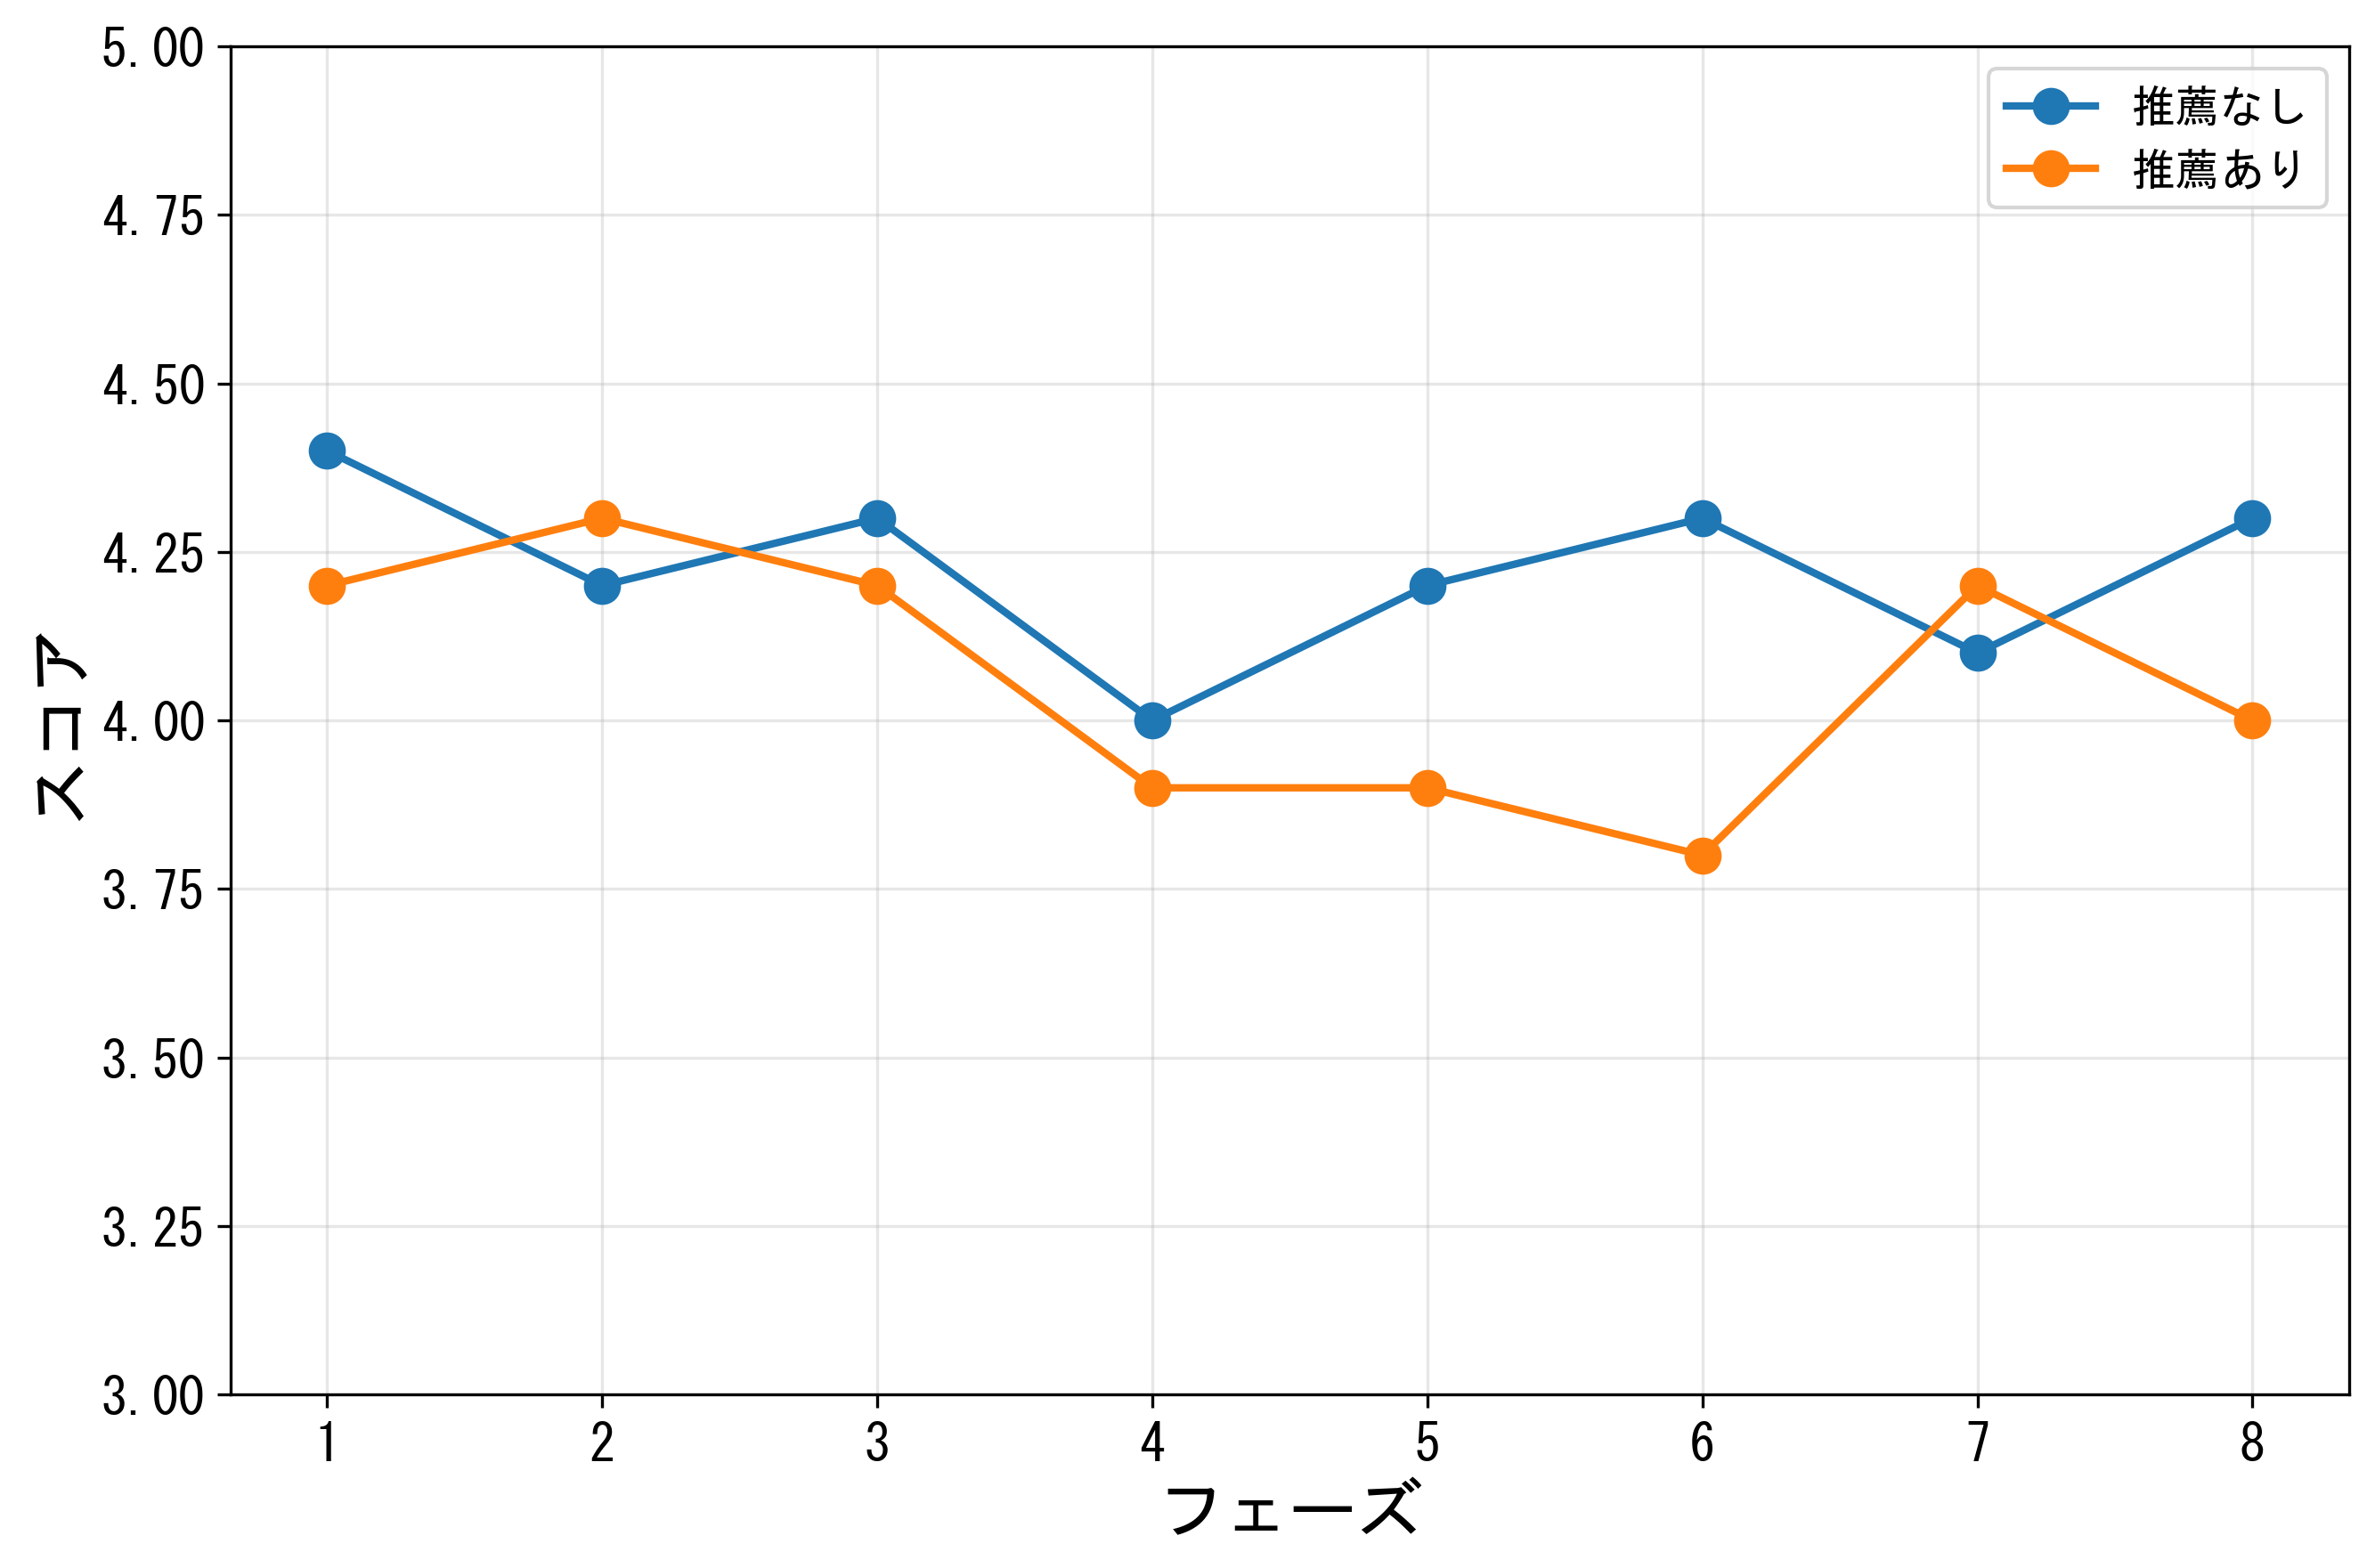
\includegraphics[width=0.9\linewidth]{image/Q6の平均推移.png}
    \caption{Q6: 相手の曲に関する思いや経験が理解できた}
    \label{fig:Q6}
\end{figure}

フェーズを独立変数，各評価項目のスコアを従属変数として単回帰分析を行った結果を表\ref{回帰係数}に示す．いずれの項目においても統計的有意差（p < 0.05）は認められなかったものの，群間で異なる傾向が観察された．推薦あり群ではEQ1（流した曲について楽しく話ができた），EQ2（自分の思いが理解してもらえた）において前半から後半にかけて正の回帰係数を示し，特にEQ5（聴いた曲について楽しく話ができた）の会話の楽しさにおいて向上傾向（β = 0.014）が確認された．これは段階的な自己開示が会話の質的向上と自己開示の受容認知の促進に寄与した可能性を示唆している．対照的に，推薦なし群ではすべての項目で負の回帰係数を示した．初期の受容度は維持されたものの自己開示のレベルが一定に留まったため，会話が表面的なものに留まり，既知の情報で会話が盛り上がってしまったことが原因であると考えられる．ただし，これらの傾向は統計的な裏付けを得るには至らず，より大規模なサンプルでの検証が必要である．

\begin{table}[H]
\caption{群ごとの自己開示の効果分析結果}
\label{回帰係数}
\begin{center}
\begin{tabular}{llcc}
\hline
立場 & 評価項目 & 群 & 回帰係数 β (p値) \\
\hline
\multirow{4}{*}{開示者} & \multirow{2}{*}{EQ1:会話の楽しさ} 
  & 推薦なし & -0.025 (0.488) \\
  & & 推薦あり & 0.080 (0.119) \\
\cline{2-4}
  & \multirow{2}{*}{EQ2:理解された実感} 
  & 推薦なし & -0.037 (0.440) \\
  & & 推薦あり & 0.051 (0.316) \\
\hline
\multirow{4}{*}{被開示者} & \multirow{2}{*}{EQ5:会話の楽しさ} 
  & 推薦なし & -0.037 (0.305) \\
  & & 推薦あり & 0.014 (0.761) \\
\cline{2-4}
  & \multirow{2}{*}{EQ6:相手への理解} 
  & 推薦なし & -0.012 (0.740) \\
  & & 推薦あり & -0.037 (0.493) \\
\hline
\end{tabular}
\end{center}
\end{table}

表\ref{table:群別の自己開示レベルごとの曲数と人数}に，各群における自己開示レベル別の集計結果を示す．この表は，各自己開示レベルについて，選曲された総数（曲数）と，そのレベルの曲を少なくとも1回選曲したユーザーの人数を示している．例えば，推薦なし群ではレベル3の曲が全体で45曲選曲され，9人のユーザーがレベル3の曲を1曲以上選んでいたことを表している．

本仮説の検証における問題として，レベル4の自己開示の出現頻度の低さが挙げられる．推薦なし群において観察されたレベル4の自己開示は全体でわずか6回に留まり，その結果，いきなり深い自己開示をしたときとの比較などを行うことができなかった．しかしながら，この現象自体が，友人関係においても最も深い自己開示が自然には起こりづらいという既存の知見を指示するものとして捉えられる．

\begin{table}[H]
  \centering
  \caption{群別の自己開示レベルごとの曲数と人数}
  \label{群別の自己開示レベルごとの曲数と人数}
  \begin{tabular}{llcccc}
    \hline
    群 & 種別 & レベル1 & レベル2 & レベル3 & レベル4 \\
    \hline
    \multirow{2}{*}{推薦なし} & 曲数[曲] & 9 & 20 & 45 & 6 \\
    & 人数[人] & 3 & 9 & 9 & 4 \\
    \hline
    \multirow{2}{*}{推薦あり} & 曲数[曲] & 17 & 23 & 30 & 10 \\
    & 人数[人] & 9 & 10 & 10 & 6 \\
    \hline
  \end{tabular}
  \label{table:群別の自己開示レベルごとの曲数と人数}
\end{table}



\subsection{仮説2の結果}\label{仮説2の結果}

\ref{研究課題と仮説}節で述べたように，仮説2は「音楽への認知度が低い，または興味度が低い場合でも，自己開示の受容度は大きく低下しない」である．
これを検証するため，EQ3（曲を知っているか）とEQ4（曲に興味を持てたか）の回答値の違いが，受容度（EQ5, EQ6）にどの程度影響を与えるか分析を行った．具体的には，EQ3（曲を知っているか）については知っている場合（1）の受容度（EQ5, EQ6）から知らない場合（0）の受容度（EQ5, EQ6）を引いた値を，EQ4（曲に興味を持てたか）については高い興味度（4-5）の受容度（EQ5, EQ6）から低い興味度（1-3）の受容度（EQ5, EQ6）を引いた値を，各ユーザーごとに算出した．表\ref{tab:differences}に各質問項目における差分の平均値と標準偏差を示す．

\begin{table}[H]
  \centering
  \begin{tabular}{ccc}
    \hline
    項目 & 平均 & 標準偏差 \\
    \hline
    各ユーザーごとのEQ3の値によるEQ5の差分 & 0.24 & 0.64 \\
    各ユーザーごとのEQ3の値によるEQ6の差分 & 0.00 & 0.72 \\
    各ユーザーごとのEQ4の値によるEQ5の差分 & 0.51 & 0.88 \\
    各ユーザーごとのEQ4の値によるEQ6の差分 & 0.23 & 0.61 \\
    \hline
  \end{tabular}
  \caption{各質問項目における差分の平均値と標準偏差}
  \label{tab:differences}
\end{table}

図\ref{EQ3比較差分のやつ}に示すように，認知度（EQ3）の影響については19名のユーザーデータを分析することができた．一方，図\ref{EQ4比較差分のやつ}に示すように，興味度（EQ4）については，興味度のスコアが1～3と，4～5が混在するユーザーは10名のみであった．

\begin{figure}[H]
    \centering
    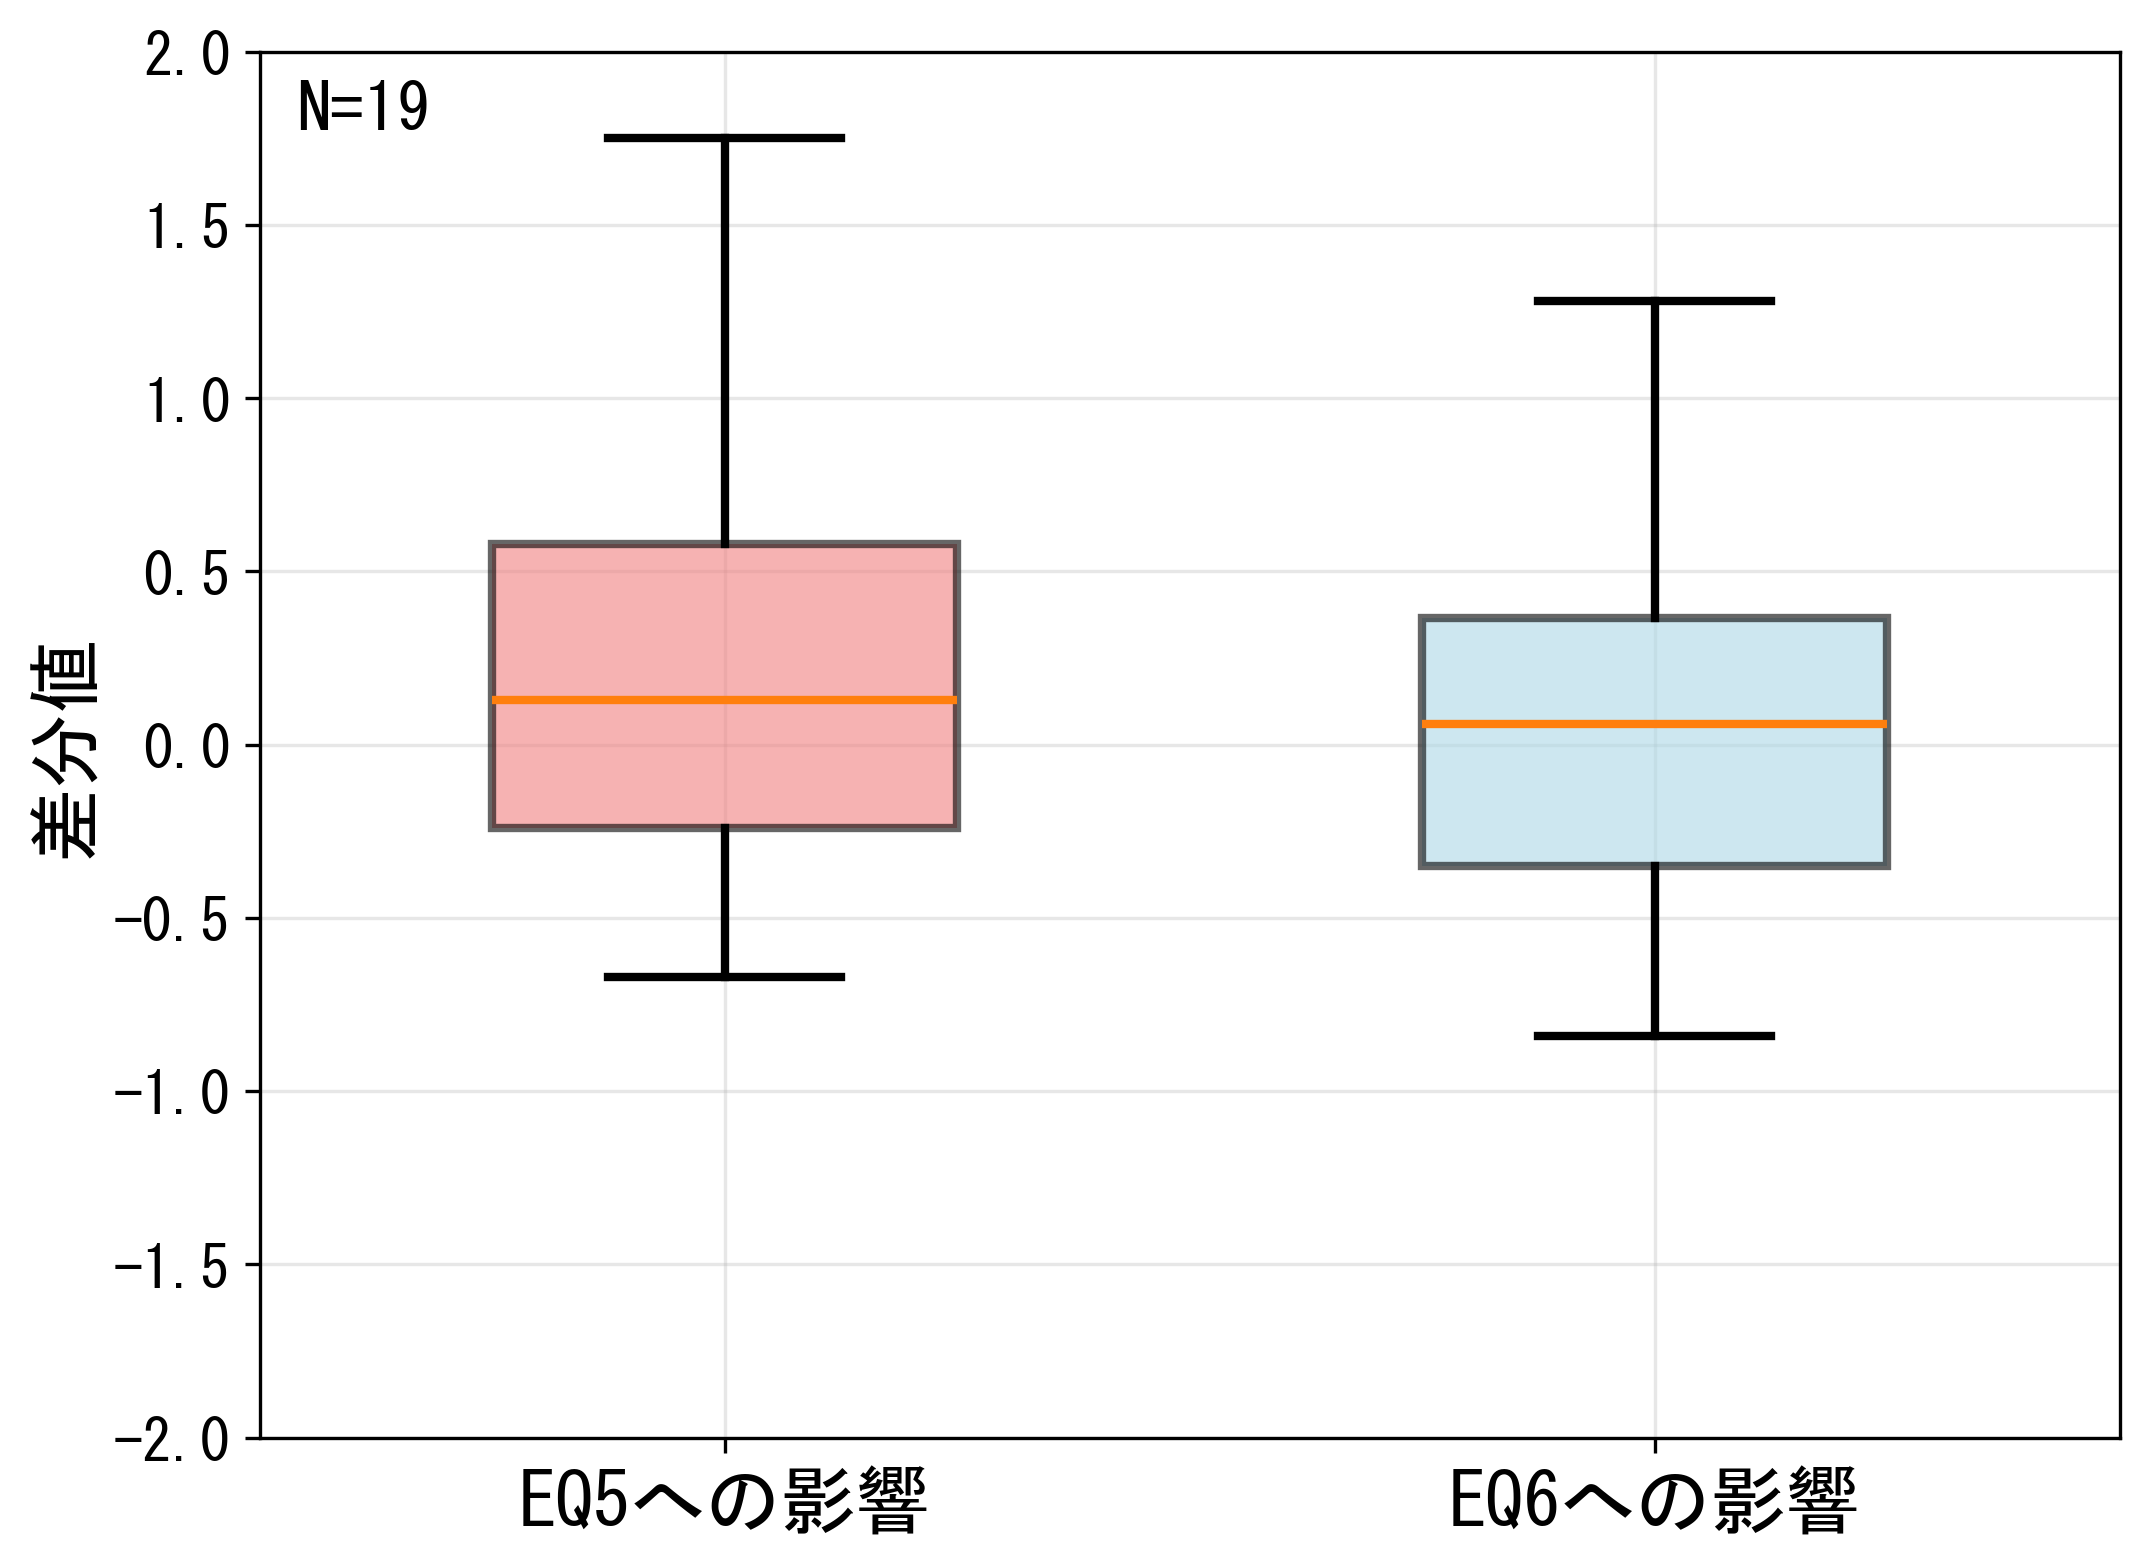
\includegraphics[width=0.75\linewidth]{image/EQ3比較差分のやつ.png}
    \caption{曲の認知度（EQ3）による受容度の差異}
    \label{EQ3比較差分のやつ}
\end{figure}

\begin{figure}[H]
    \centering
    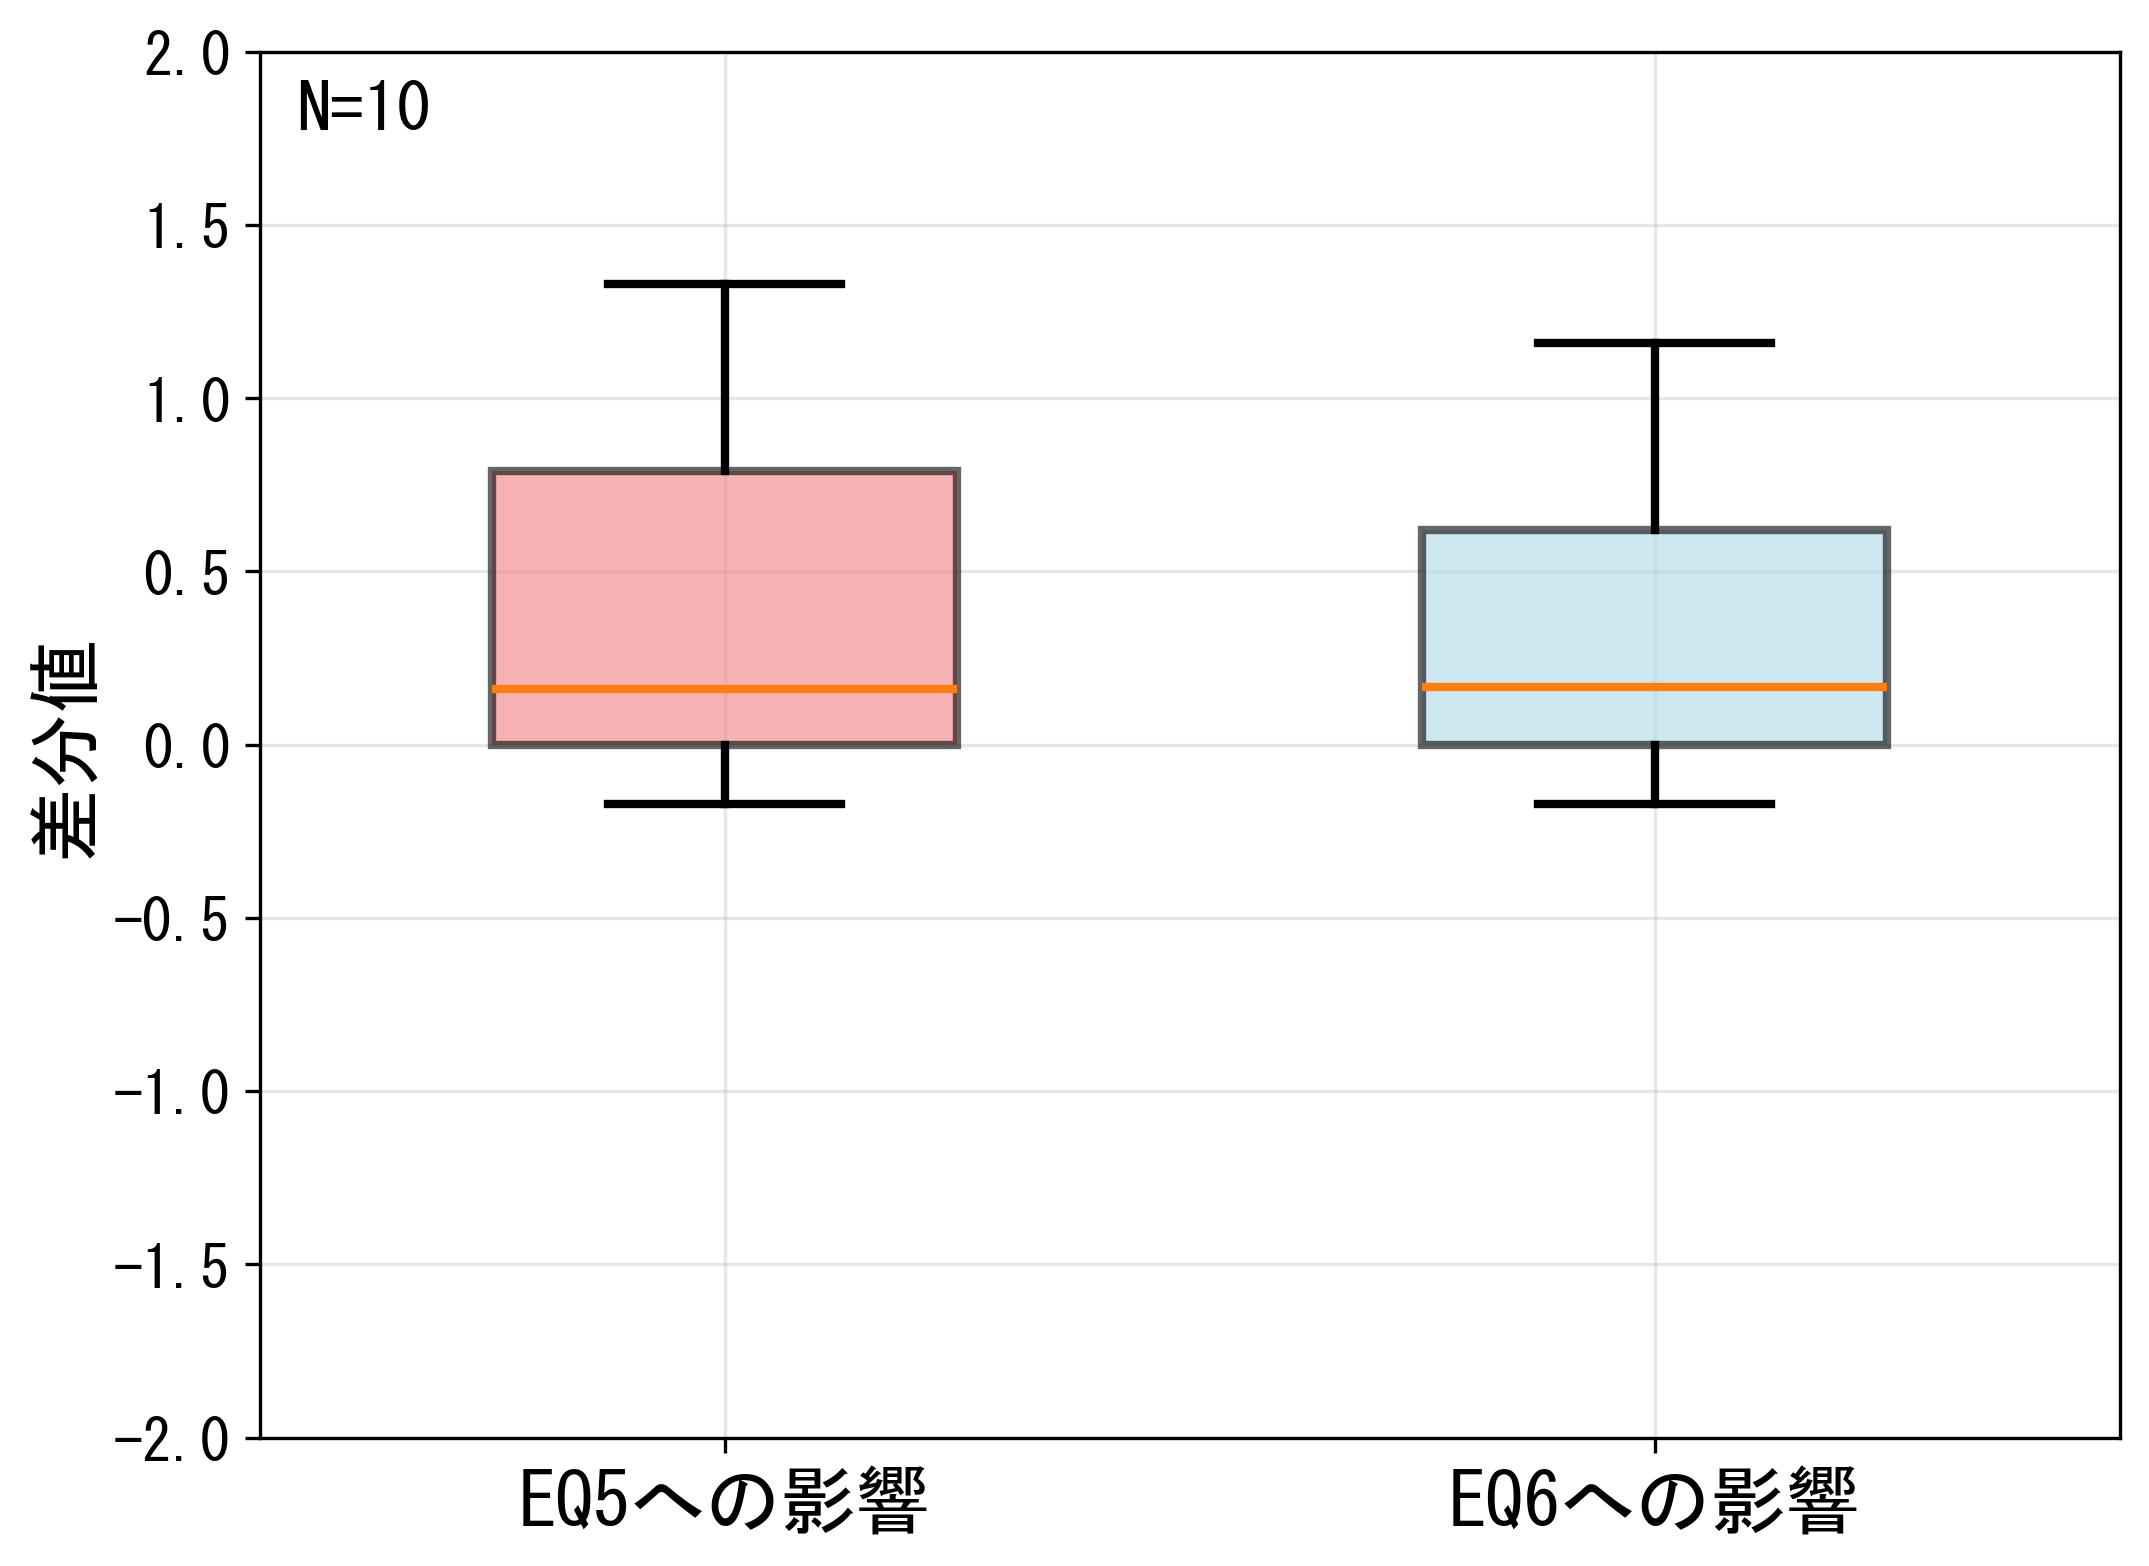
\includegraphics[width=0.75\linewidth]{image/EQ4比較差分のやつ.png}
    \caption{曲の興味度（EQ4）による受容度の差異}
    \label{EQ4比較差分のやつ}
\end{figure}

認知度（EQ3）の影響について，表\ref{tab:differences}に示すように，EQ5（聴いた曲について楽しく話ができた）とEQ6（思いや経験が理解できた）への差分平均値はそれぞれ0.24（標準偏差0.64）と0.00（標準偏差0.72）となった．図\ref{EQ3比較差分のやつ}から分かるように，EQ5（聴いた曲について楽しく話ができた）への影響はプラスの傾向を示すものの，データの分布は比較的狭い範囲に収まっている．EQ6（思いや経験が理解できた）への影響はさらに顕著で，中央値がほぼ0に近く，データのばらつきも小さいことから，曲の認知度が相手の思いや経験の理解にほとんど影響を与えていないことを示している．

次に，興味度（EQ4）の影響については，10名のデータを分析した結果，EQ5（聴いた曲について楽しく話ができた）とEQ6（思いや経験が理解できた）への差分平均値がそれぞれ0.51（標準偏差0.88）と0.23（標準偏差0.61）となった．図\ref{EQ4比較差分のやつ}から分かるように，両方の指標において極端な負の値は見られず，中央値も近い値を示している．
% 特にEQ5への影響については，データの大部分が正の値を示しており，興味度が高い場合の方が受容度が高い傾向があることが示唆された．
ただし，EQ5（聴いた曲について楽しく話ができた）については標準偏差が大きいことから，データのばらつきが大きく，この傾向は個人差が大きいことが確認された．つまり，興味度の高低が受容度に与える影響は一概に判断できないと考えられる．

興味度と認知度の両方において，値にばらつきは見られるものの四分位範囲は比較的小さく，極端な正負の値も少ないことから，多くのユーザーで安定した結果が得られたと言える．つまり，相手の曲を知らない，あるいは強い興味を持っていない場合であったとしても，自己開示に対する受容度は大きく低下しないことが示された．このことは，音楽への興味度や知識が自己開示の受容に与える影響が限定的であることを示唆している．以上の分析結果から，仮説2「被開示者の音楽への興味度に関わらず，高い受容度を示す」については支持されたと考えられる．



\subsection{仮説3の結果}\label{仮説3の結果}

\ref{研究課題と仮説}節で述べた仮説3「セッションを終えた2者は，段階的に自己開示を促していない方に比べて相手に対する受容性が向上する」について検証を行った．
実験後のアンケートを平均値にした図\ref{fig:事後アンケート}では，全項目について推薦あり群より推薦なし群の方が満足度が高く，特にPQ6（実験前より相手の音楽の好みについて理解できた）は推薦なし群の方が1ポイントほど高いことが分かる．これは，セッション内での自己開示レベルの高い曲への受容性は向上していたものの，序盤は自己開示レベルの低い曲しか選曲できなかったことから，全体を通して深い自己開示があまりできず，相互理解の促進に繋がらなかったのではないかと考えられる．

推薦なし群と推薦あり群の間で評価値の分布に有意な差があるかを検討するために，Mann-WhitneyのU検定を行った．すると，PQ6の項目においてのみ有意な差（U = 83.000, p = 0.006, r = .609）が見られた．
しかし，PQ5（U = 53.500, p = 0.805, r = .055）およびPQ7（U = 61.500, p = 0.335, r = .216）では有意な差は見られなかった．両項目において，両群ともに高い評価値（4ポイント以上）を示しており，これは推薦システムの有無に関わらず，音楽を介した対話が相互理解と音楽を通じたコミュニケーションの意欲を促進する可能性を示唆している．

\begin{figure}[H]
    \centering
    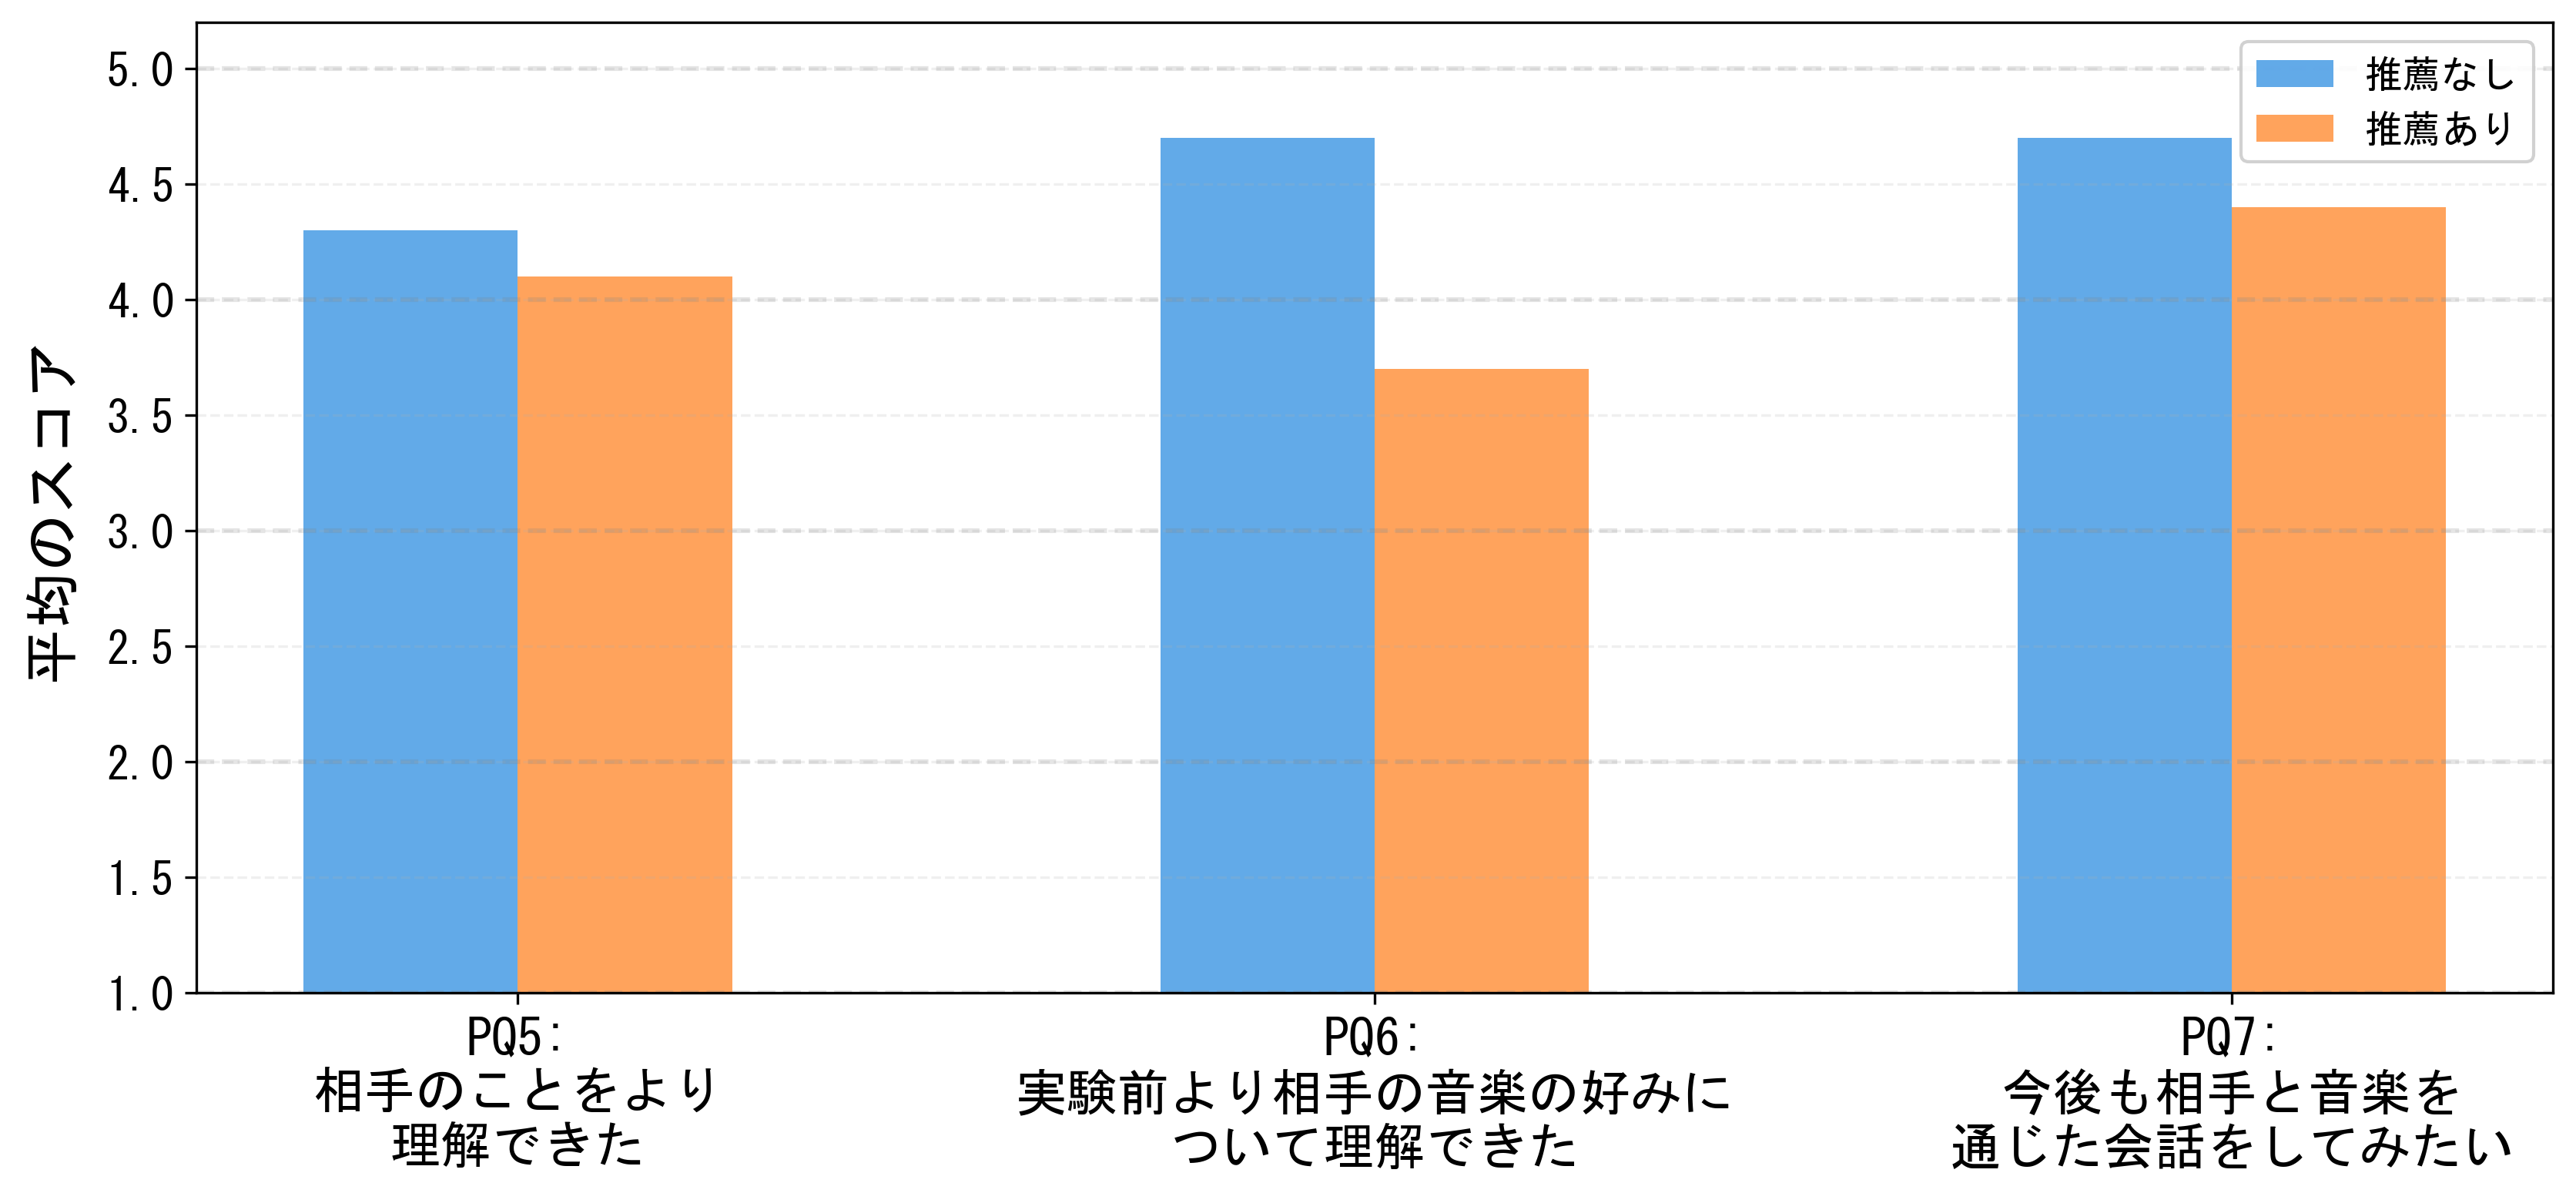
\includegraphics[width=1\linewidth]{image/実験後の受容質問3つ.png}
    \caption{実験後アンケート結果の比較}
    \label{fig:事後アンケート}
\end{figure}


各被験者の実験後アンケート結果を，表\ref{fig:実験後アンケート表}に示す．多くの被験者がPQ5（相手のことをより理解できた），PQ6（実験前より相手の音楽の好みについて理解できた），PQ7（今後も相手と音楽を通じた会話をしてみたい）の3項目について4点または5点の高評価を示した中で，特徴的な回答が見られた．

推薦あり群のアンケートの平均値が下がった理由として，ペア3の結果が挙げられる．
ペア3は他のペアと比較して顕著に低い評価が観察され，特に被験者Fの回答（PQ5：3点，PQ6：1点，PQ7：3点）は全被験者の中で特に低い値を示した．被験者FのPQ4（自分の内面についてよく話すことができた）で1点を示しているように，ヒアリングから，音楽についてうまく話せないことに苛立ちを覚えて，自己嫌悪し，空気を悪くしてしまったことが明らかになった．一方で，システムによる推薦に対しての不満はなく，被験者Eからは「どの曲も話した過ぎて何を選ぶか悩んだ」という報告があり，段階的な推薦は悪影響を及ぼしていないことが確認された．

対照的に，推薦あり群のペア10については，普段からよく音楽の話をしているが，様々なジャンルについて触れて話ができたり，相手のことを深く知ることができたと答えていた．システムが提示した4つの選択肢には，いずれも対話の題材として魅力的な楽曲が含まれており，選曲の意思決定にポジティブな迷いが生じたことが報告された．このことは，システムによる楽曲推薦が有効な選択肢を提供できていたことを示唆している．

さらに，ヒアリングの結果，推薦なし群からは「相手の音楽の趣味が思ったより異なることが分かった」「相手の好きな音楽についてより深く理解できた」といった音楽嗜好の表面的な理解に関する言及が多く見られた．一方で，推薦あり群からは「相手のことを深く知ることができた」「なぜ曲を好きになったか，曲に対する熱意を知れた」など，音楽を通じた個人的な思い出や背景についての言及がされていた．この結果は，段階的な音楽推薦システムが，単に音楽の好みを共有するだけでなく，被験者間のより深い相互理解の形成に寄与する可能性を示している．


\begin{figure}[H]
    \centering
    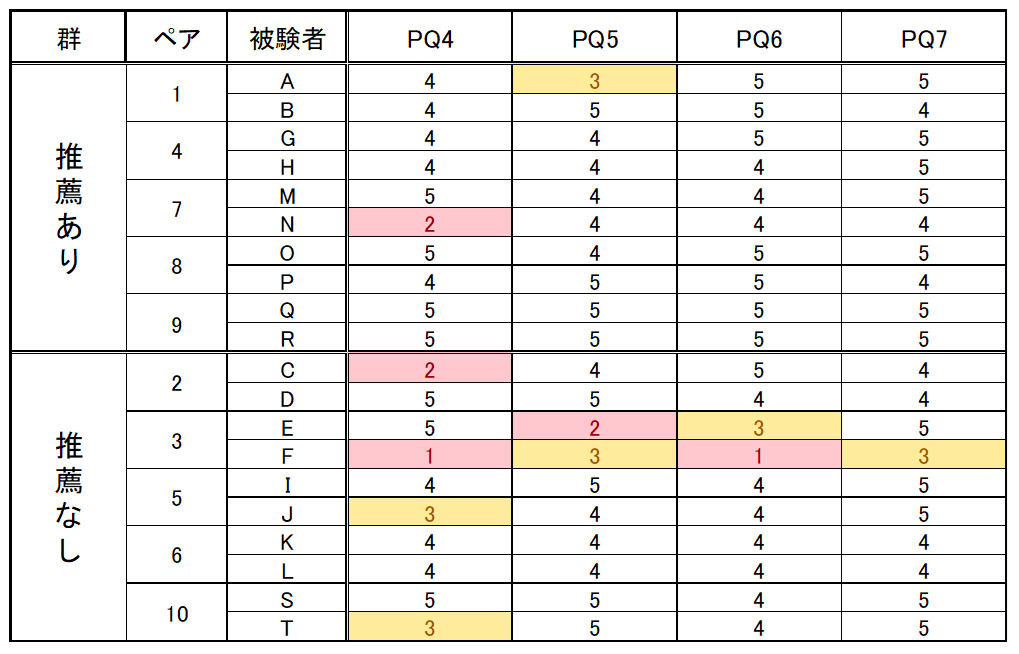
\includegraphics[width=0.9\linewidth]{image/実験後アンケート表2.png}
    \caption{被験者ごとの実験後アンケート（PQ4～PQ7）}
    \label{fig:実験後アンケート表}
\end{figure}


\begin{comment}
    実験序盤から終盤での差異を見るため，EQ5, EQ6について，後半フェーズ（7～8）の平均値から前半フェーズ（1～2）の平均値を減算し，その変化量を算出した．その結果を図\ref{fig:EQ5-最初to最後の変化量}, 図\ref{fig:EQ6-最初to最後の変化量}に示す．
    
    EQ5については，推薦あり群では平均0.20ポイントの向上が見られたが，推薦なし群では平均-0.15ポイントの低下が確認された．また，標準偏差は推薦あり群（0.632）の方が推薦なし群（0.973）より小さく，段階に推薦をすることによって，より安定した効果が得られたことが示唆された．
    一方，EQ6については，推薦なし群（標準偏差0.775）および推薦あり群（標準偏差0.626）の両群において，平均値では若干の低下傾向が観察された．しかし，分布の形状に着目すると，推薦あり群ではデータの上部が正の値まで広く分布しているのに対し，推薦なし群では上方への広がりが小さかった．この分布の特徴は，段階的推薦を受けた推薦あり群において，一部のペアでは相手への理解が深まる可能性があることを示唆している．また，推薦あり群では，全体としては若干の低下傾向を示しているものの，データの上部が正の方向に広く分布しており，個人差はあるものの相手理解の促進に対して良い効果が得られる可能性が示唆された．
    
    \begin{figure}[H]
        \centering
        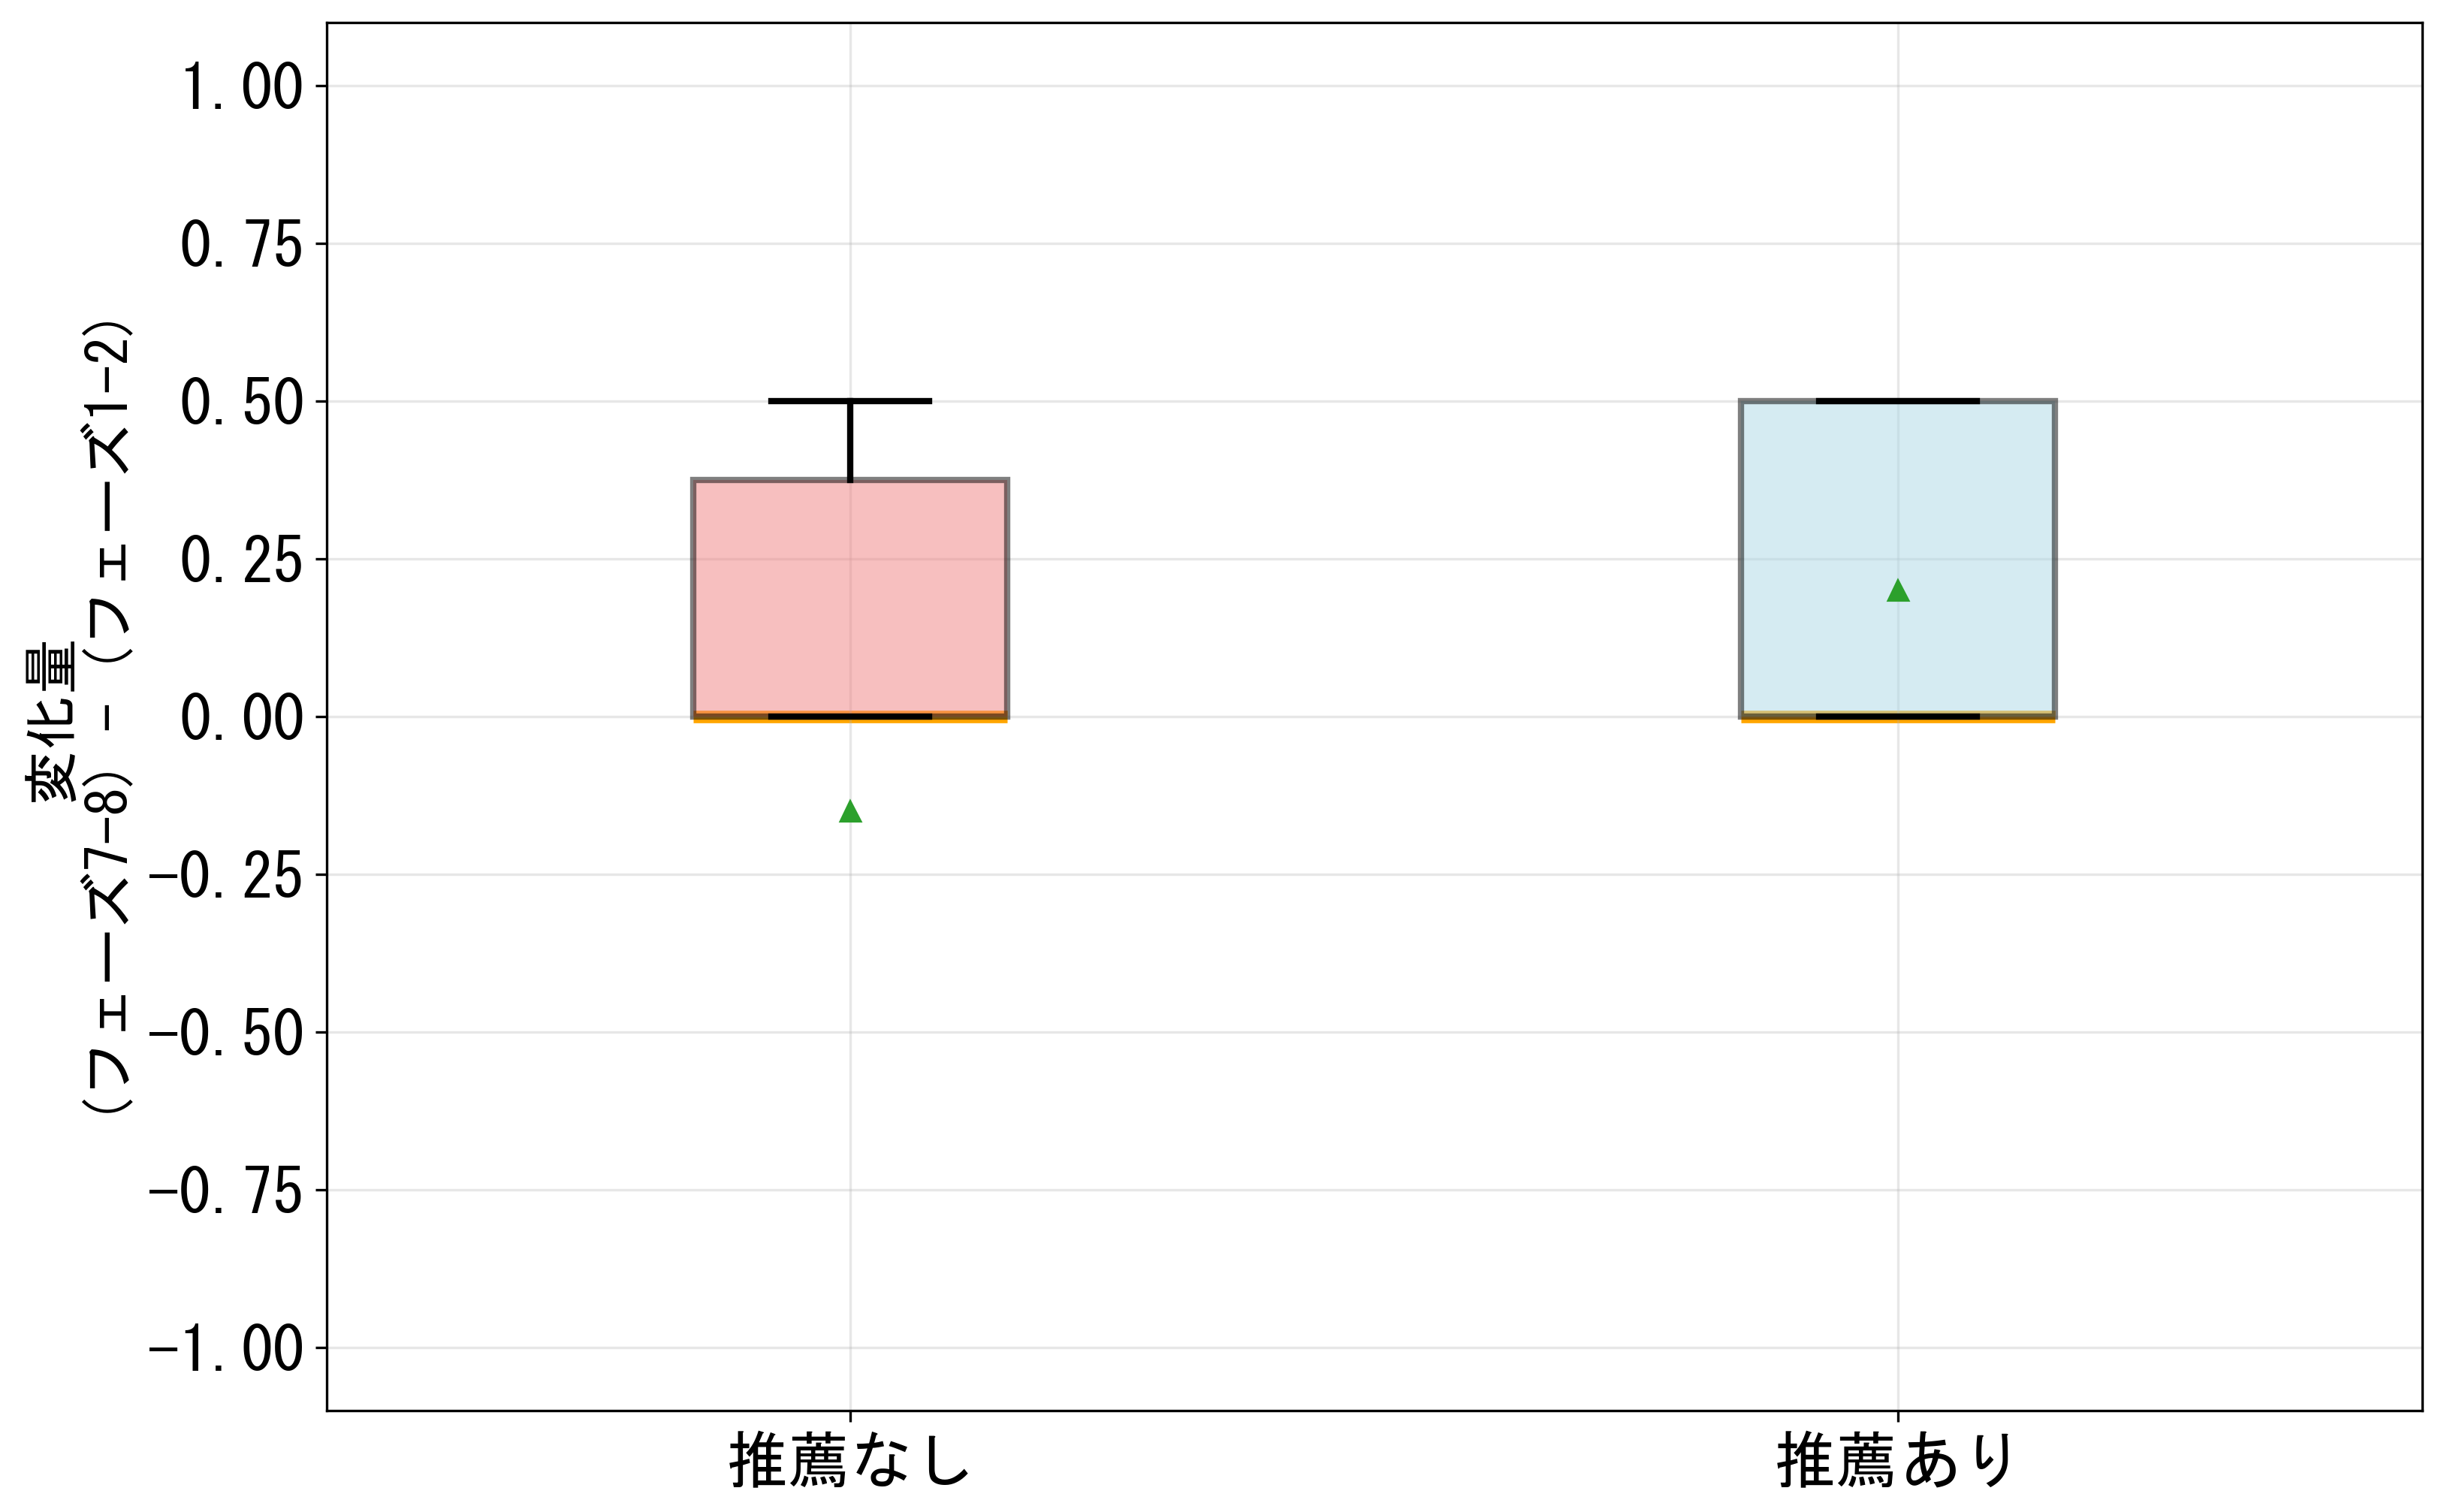
\includegraphics[width=0.9\linewidth]{image/EQ5_最終と序盤の差異_Box.png}
        \caption{EQ5: 序盤(フェーズ1-2)から終盤(フェーズ7-8)の変化量}
        \label{fig:EQ5-最初to最後の変化量}
    \end{figure}
    
    \begin{figure}[H]
        \centering
        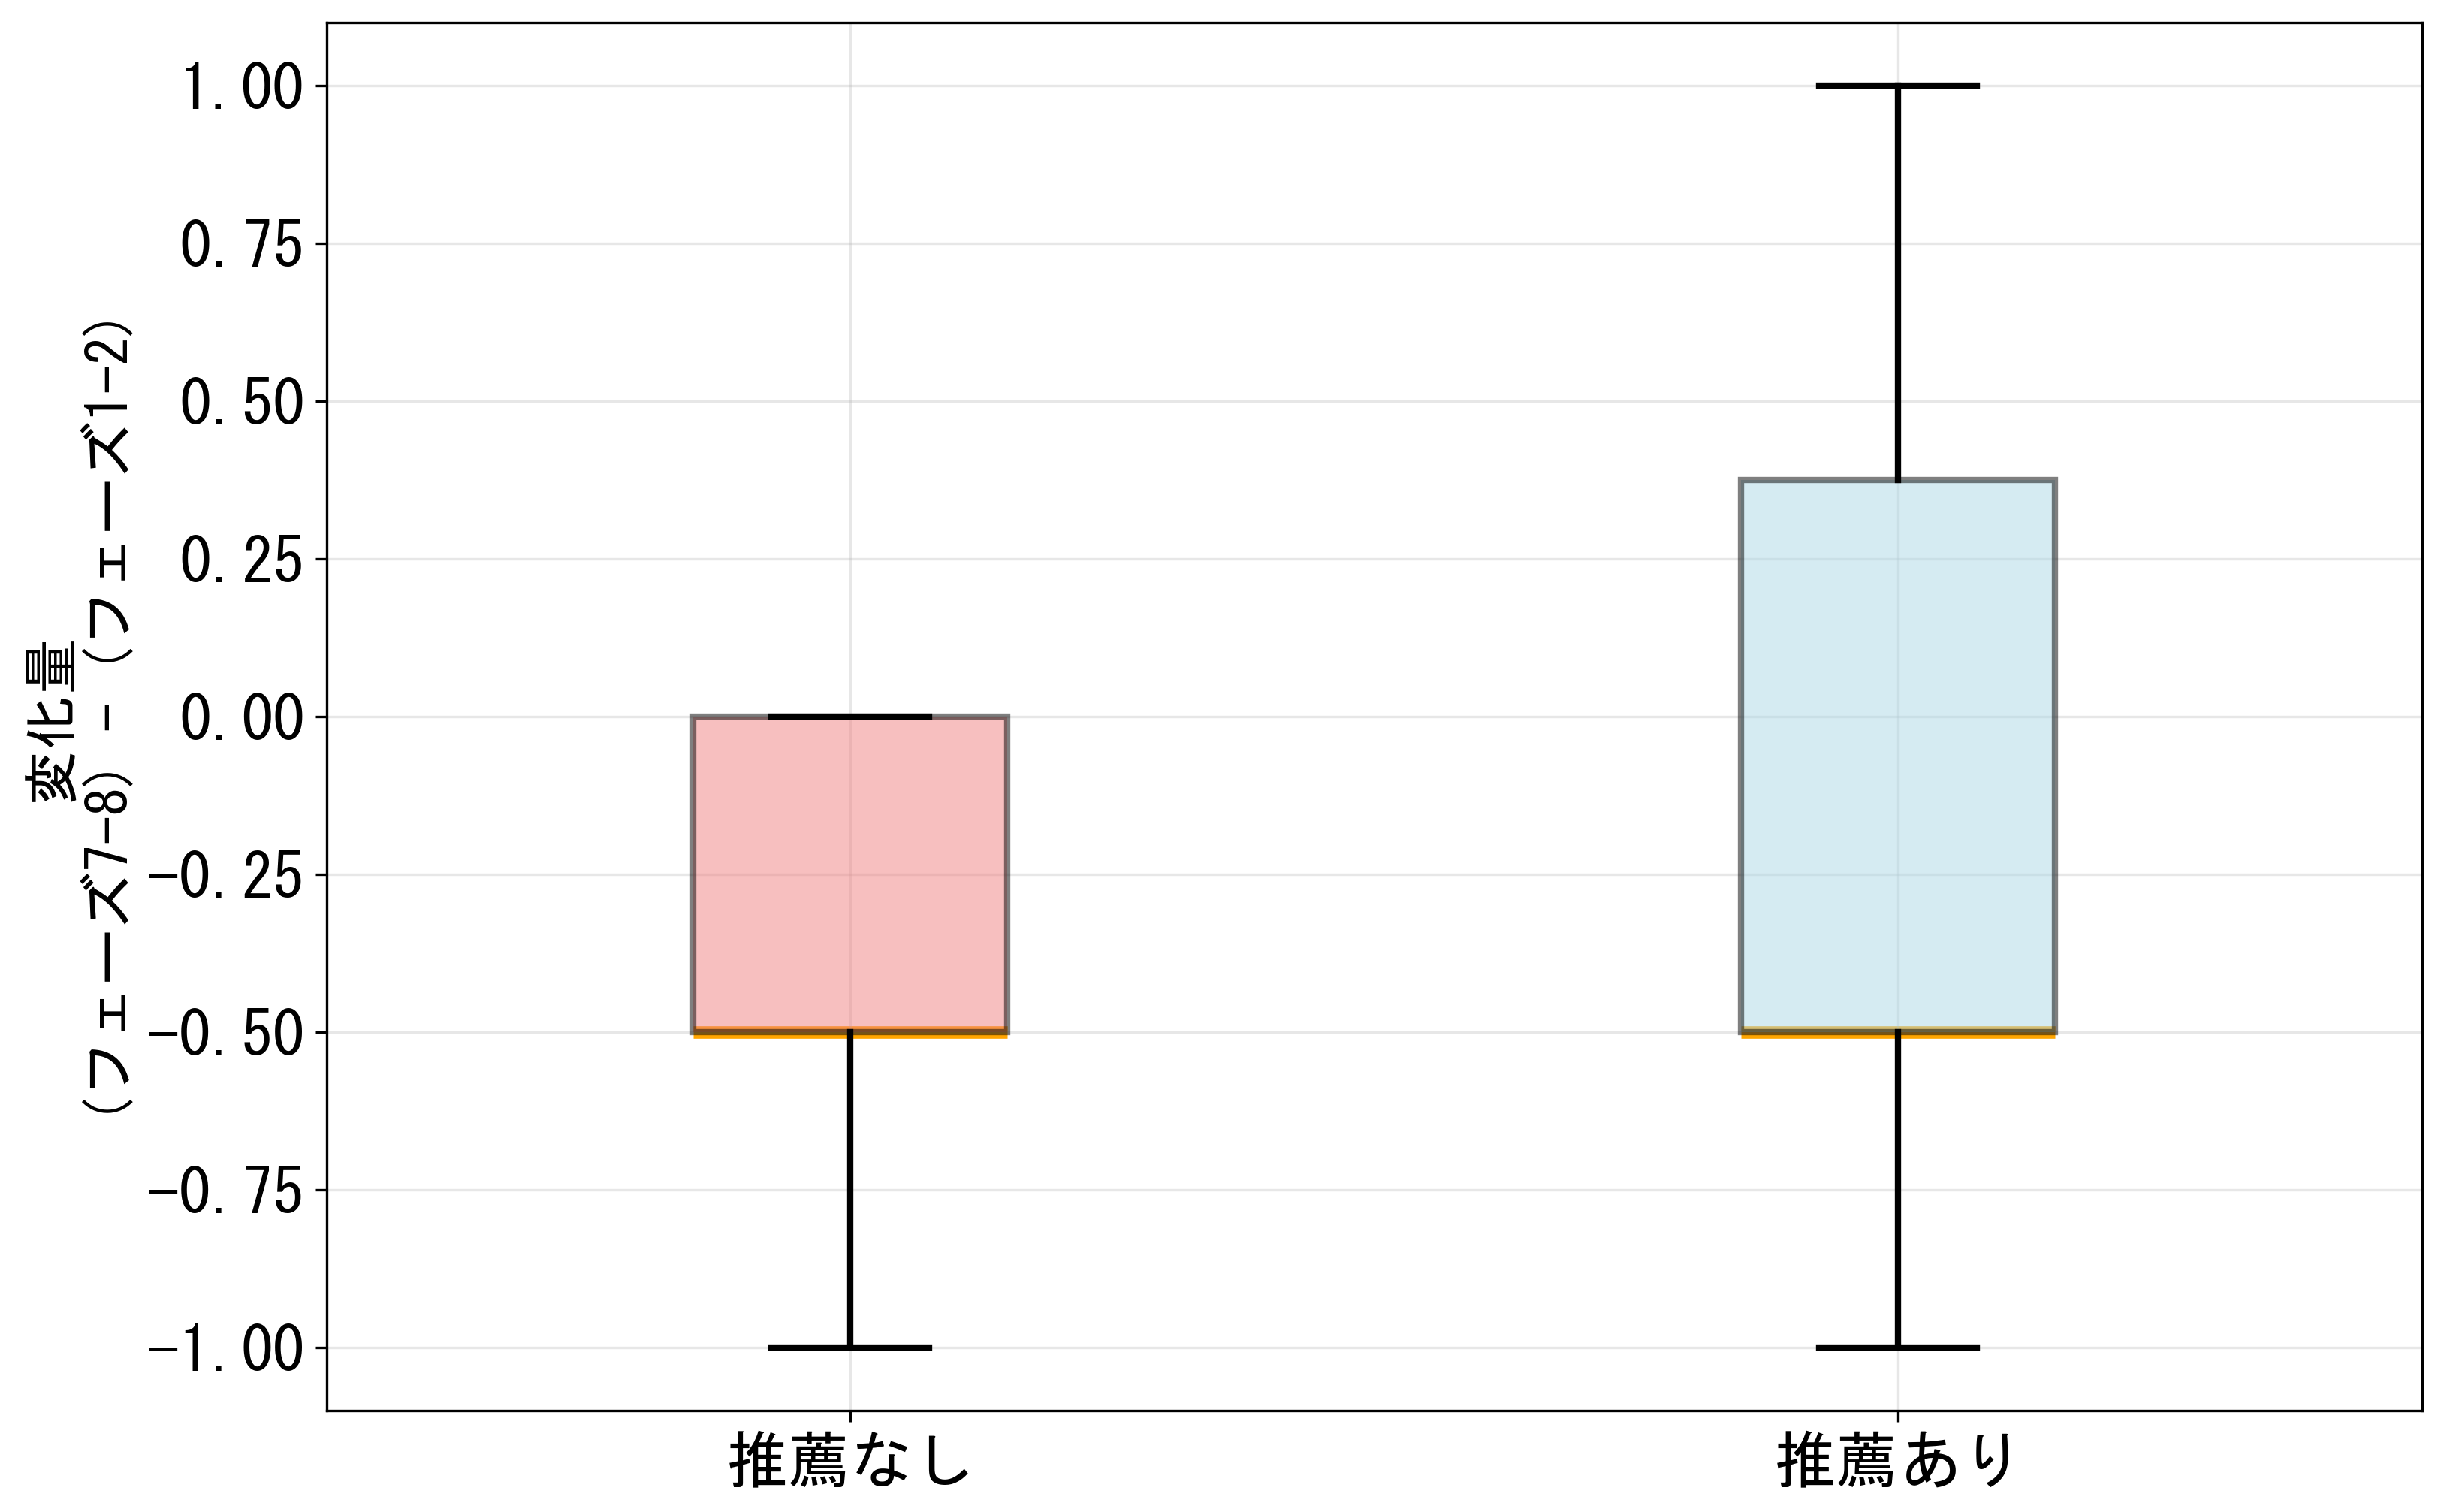
\includegraphics[width=0.9\linewidth]{image/EQ6_最終と序盤の差異_Box.png}
        \caption{EQ6: 序盤(フェーズ1-2)から終盤(フェーズ7-8)の変化量}
        \label{fig:EQ6-最初to最後の変化量}
    \end{figure}
\end{comment}
